%% Signal, Image and Video Processing — Springer Nature
%% sn-jnl document class, mathphys-num style, two-column layout
\documentclass[pdflatex,sn-mathphys-num,iicol]{sn-jnl}

%%%% Standard Packages
\usepackage{bookmark}
\usepackage{tabularx}
\usepackage{diagbox}
\usepackage{tikz}
\usetikzlibrary{shapes.geometric, arrows.meta, positioning, calc, fit, backgrounds}

\usepackage{graphicx}%
\usepackage{multirow}%
\usepackage{amsmath,amssymb,amsfonts}%
\usepackage{amsthm}%
\usepackage{mathrsfs}%
\usepackage[title]{appendix}%
\usepackage{xcolor}%
\usepackage{textcomp}%
\usepackage{manyfoot}%
\usepackage{booktabs}%
\usepackage{algorithm}%
\usepackage{algorithmicx}%
\usepackage{algpseudocode}%
\usepackage{listings}%
%%%%

\theoremstyle{thmstyleone}%
\newtheorem{theorem}{Theorem}%
\newtheorem{proposition}[theorem]{Proposition}%

\theoremstyle{thmstyletwo}%
\newtheorem{example}{Example}%
\newtheorem{remark}{Remark}%

\theoremstyle{thmstylethree}%
\newtheorem{definition}{Definition}%

\raggedbottom

\begin{document}

%% -----------------------------------------------------------------------
%%  TITLE AND AUTHORS
%% -----------------------------------------------------------------------

\title[CQT Feature Robustness under Acoustic Domain Shift]{%
Evaluating Constant-Q Transform Feature Robustness and Classifier
Generalization under Acoustic Domain Shift: A CNN-SVM Comparative Study
on Piano Chord Recognition}

\author*[1]{\fnm{Cikal} \sur{Gemintang Seya}}%
  \email{cikal.gemintang@mhs.itenas.ac.id}

\author[1]{\fnm{Jasman} \sur{Pardede}}%
  \email{jasman@itenas.ac.id}

\affil*[1]{%
  \orgdiv{Informatics},
  \orgname{Institut Teknologi Nasional Bandung},
  \orgaddress{%
    \street{Neglasari},
    \city{Bandung},
    \postcode{40124},
    \state{West Java},
    \country{Indonesia}}}

%% -----------------------------------------------------------------------
%%  ABSTRACT
%% -----------------------------------------------------------------------

\abstract{%
Spectral feature representations derived from audio signals are widely used
as 2D image inputs to convolutional classifiers, yet the generalization
behaviour of these features and their downstream classifiers under acoustic
domain shift remains insufficiently characterised.
This paper presents a systematic study of Constant-Q Transform (CQT)
spectrogram features paired with two fundamentally different classifiers—a
Convolutional Neural Network (CNN) and a hyperparameter-tuned
Radial Basis Function Support Vector Machine (RBF-SVM)—evaluated on a
controlled 36-class piano chord recognition problem.
Both classifiers are trained on a dataset of 7,200 audio samples recorded
from a Techno T-9890i keyboard and subsequently tested on a separate,
independent 1,440-sample dataset recorded from a Yamaha PSR-S910
keyboard in a different physical environment, constituting an explicit
cross-domain evaluation protocol.
Under within-distribution 5-fold cross-validation, both models achieve
perfect accuracy (1.00) and F1-score (1.00), confirming that CQT features
are fully discriminative for this vocabulary under controlled conditions.
The decisive finding emerges under cross-domain testing: the CNN retains
strong generalisation with 0.89 accuracy and 0.87 macro F1-score, whereas
the SVM collapses to 0.29 accuracy and 0.36 macro F1-score, defaulting
to single-class prediction for the large majority of test inputs.
Analysis of misclassification patterns reveals that the CNN's residual
errors are concentrated in a small set of harmonically proximate chord
pairs, whereas the SVM exhibits a systematic attractor failure caused by
global spectral envelope shift in the kernel distance metric.
These results provide empirical evidence that CNN's spatially local,
hierarchical feature learning is substantially more robust to inter-device
and inter-instrument acoustic variation than the global kernel boundary of
RBF-SVM, a finding with broader implications for the deployment of
spectrogram-based classifiers beyond the specific domain of music.}

\keywords{%
Constant-Q Transform, Feature Generalisation, Domain Shift,
Convolutional Neural Network, Support Vector Machine, Spectrogram
Classification, Acoustic Robustness}

\maketitle

%% -----------------------------------------------------------------------
\section{Introduction}\label{sec1}
%% -----------------------------------------------------------------------

Spectrogram-based image classification has become a dominant paradigm
across diverse audio recognition tasks, including environmental sound
classification \cite{Wolf-Monheim2025}, speech recognition
\cite{Zaman2023}, and music analysis \cite{Moysis2023}.
In this paradigm, a time-frequency representation of an audio signal is
treated as a 2D image and processed by a convolutional classifier, a
strategy that exploits the well-established strength of convolutional
neural networks (CNNs) in learning spatially local, hierarchical
feature representations.
A critical but often under-examined question concerns how robustly the
learned feature-classifier system generalises when the acoustic recording
conditions at test time differ from those at training time — a situation
routinely encountered in practical deployment.

This mismatch, broadly termed \emph{acoustic domain shift}, arises
whenever characteristics such as instrument timbre, microphone frequency
response, room acoustics, or recording device differ between the training
corpus and the deployment environment \cite{Kusaka2024} \cite{Majchrzak2025}.
Under such conditions, a feature representation that is perfectly
discriminative in-distribution may lose discriminative power
out-of-distribution, and a classifier whose decision boundary is
optimally placed in the training feature space may become
misaligned in the shifted feature space.
Understanding which combinations of spectral feature representations
and classifier architectures are robust to such shifts is therefore
of substantial practical and theoretical importance.

Among time-frequency representations, the Constant-Q Transform (CQT)
occupies a particular position: its logarithmically spaced frequency
bins are aligned to the chromatic musical scale \cite{Li2021}
\cite{Lacoste2007}, which means that harmonic overtone structures—the
dominant spectral feature of musical sounds—appear as translationally
consistent patterns across the frequency axis regardless of instrument
register.
This structural alignment makes CQT spectrograms a natural testbed
for investigating feature robustness, since the fundamental pattern
of interest (harmonic interval structure) is geometrically stable,
while secondary factors such as timbre, loudness, and recording
device frequency response produce global and local distortions of that
pattern \cite{Li2021} \cite{Telila2023}.

The piano chord classification problem provides a controlled and
systematically varied vocabulary for such a study.
With 36 classes organised as 12 chromatic root notes times 3 chord
qualities (major, minor, diminished), the task requires fine-grained
spectral discrimination: major and minor triads differ by a single
semitone shift in the third, and diminished triads differ by a further
single semitone shift in the fifth, corresponding to shifts of one or
two CQT frequency bins at the chosen resolution.
The problem is therefore neither trivially easy (the classes are
harmonically close) nor artificially hard (the features are
geometrically regular), making it an appropriate benchmark for
comparative generalisation analysis.

The two classifier architectures evaluated in this study, CNN and
RBF-SVM, represent opposing strategies for learning decision boundaries
in feature space.
CNN learns a spatially localised, hierarchical feature detector:
convolutional kernels respond to small neighbourhoods in the
time-frequency plane, and deep stacking builds progressively abstract
representations \cite{OShea2015} \cite{Purwono2022}.
RBF-SVM learns a maximum-margin hyperplane defined by kernel similarity
to a set of training support vectors, where the RBF kernel measures the
global Euclidean distance between flattened feature vectors
\cite{Chang2011} \cite{Wainer2020}.
Under acoustic domain shift, these two strategies are expected to behave
very differently: the CNN's locally defined representations should
remain partially invariant to global spectral shifts, whereas the
SVM's globally defined kernel distances may be severely distorted by
the same shifts \cite{Zaman2023}.

The existing literature on audio classification generalisability
reveals several gaps.
The majority of published chord recognition systems focus on
large-vocabulary offline recognition using complex architectures such
as CNN-HMM hybrids \cite{Li2021}, CNN-RNN hybrids \cite{OHanlon2021},
conformer-based models \cite{Akram2025}, or transformer-attention
mechanisms \cite{Akram2025} \cite{Kusaka2024}, and are evaluated on
within-distribution test splits or standardised benchmarks that do not
probe cross-dataset generalisation.
Comparative evaluations of CNN against kernel-based classifiers specifically
under acoustic domain shift are notably absent.
Studies that do address domain shift in audio classification typically
employ data augmentation or domain adaptation strategies rather than
examining the root cause of classifier brittleness
\cite{Majchrzak2025} \cite{Kusaka2024}.

This paper addresses these gaps with a controlled experimental design
in which the training and evaluation datasets are recorded on different
keyboard instruments (Techno T-9890i and Yamaha PSR-S910) with
different synthesis algorithms and different recording devices, in
different physical environments, while all other parameters (chord
vocabulary, sample count, note timing variation) are systematically
controlled.
This setup explicitly isolates the effect of acoustic domain shift and
enables a rigorous comparison of feature-classifier generalisation
capacity.

The specific contributions of this work are as follows:

\begin{enumerate}[1.]

\item An experimental demonstration that CQT spectrograms are fully
discriminative for 36-class piano chord classification under
within-distribution conditions, confirmed by perfect accuracy and
F1-score from both CNN and RBF-SVM across 5-fold cross-validation.

\item A cross-domain evaluation protocol using two independently
recorded keyboard datasets that differ in instrument, synthesis
algorithm, recording device, and physical environment, providing a
controlled benchmark for acoustic domain shift generalisation analysis.

\item A comparative evaluation showing that CNN and RBF-SVM are
equivalent under within-distribution evaluation but exhibit
sharply divergent behaviour under acoustic domain shift: the CNN
achieves 0.89 accuracy and 0.87 macro F1-score on the unseen
evaluation dataset, whereas the RBF-SVM collapses to 0.29 accuracy
and 0.36 macro F1-score.

\item A detailed analysis of classifier failure modes: CNN misclassifications
follow systematic harmonic proximity patterns concentrated in a small
number of chord pairs, whereas SVM failure is characterised by a global
attractor collapse in which the majority of test samples are mapped
to a single class — an outcome attributable to spectral envelope shift
in the RBF kernel distance metric.

\item Empirical evidence supporting the broader claim that spatially local,
hierarchical feature learning (CNN) is more robust to acoustic covariate
shift than global kernel boundary learning (RBF-SVM), a finding
generalising beyond the specific domain of music to any application
involving spectrogram-based classification.

\end{enumerate}

%% -----------------------------------------------------------------------
\section{Related Work}\label{sec2}
%% -----------------------------------------------------------------------

\subsection{Spectrogram-Based Audio Classification}\label{subsec2_1}

The use of time-frequency spectrograms as 2D image inputs to
convolutional classifiers has become a standard approach across
audio classification tasks.
Zaman et al.\ \cite{Zaman2023} provide a comprehensive survey of deep
learning methods for audio signal classification, covering CNN, RNN,
autoencoder, transformer, and hybrid architectures across speech, music,
and environmental sound domains.
Their survey establishes the CNN-spectrogram pipeline as the dominant
methodology and identifies distribution shift as a key open challenge
across all audio classification sub-domains.
Moysis et al.\ \cite{Moysis2023} specifically survey deep learning
applications in music signal processing, confirming that CNN architectures
applied to spectral features routinely achieve higher accuracy than other
feature representations in controlled evaluation settings.

Wolf-Monheim \cite{Wolf-Monheim2025} conducted a systematic comparison of
spectral and rhythmic features — including mel-scaled spectrograms,
MFCCs, STFT chromagrams, CQT chromagrams, and CENS chromagrams — for
audio category and class level classification using a deep CNN on the
ESC-50 dataset.
Their results demonstrate that feature choice substantially affects
classification performance, with mel-scaled spectrograms and MFCCs
outperforming other representations in controlled environmental sound
classification.
A key implication of this work is that feature choice and classifier
architecture must be evaluated jointly, not independently, and that
rankings may reverse under different evaluation conditions.

Bartusiak and Delp \cite{Bartusiak2022} demonstrated that
frequency-domain spectrogram CNN classifiers can achieve high accuracy
for synthetic versus genuine audio discrimination, highlighting the
discriminative capacity of spectral image representations even for
subtle inter-distribution differences, a capacity that is directly
relevant to the cross-instrument evaluation performed in this study.

\subsection{CQT Features for Musical Audio Analysis}\label{subsec2_2}

The Constant-Q Transform's logarithmically spaced frequency bins,
aligned to the chromatic musical scale, make it particularly well-suited
for music audio analysis \cite{Li2021} \cite{Lacoste2007}.
Li \cite{Li2021} conducted a systematic comparison of CQT, STFT, and
CENS features as inputs to CNN and DNN classifiers for chord recognition,
reporting that CQT features yielded the highest individual accuracy
of 84.2\% on the CNN model, compared to 75.3\% for STFT and 80.8\%
for CENS.
This established CQT as the preferred spectral feature for CNN-based
chord classification and directly motivates its use in the present study.

Telila et al.\ \cite{Telila2023} applied a CNN-CQT pipeline to
polyphonic piano automatic music transcription, achieving frame-level
accuracy of 88.2\% and demonstrating that the CQT representation
captures the frequency structure of piano notes effectively when
combined with convolutional feature learning.
O'Hanlon and Sandler \cite{OHanlon2021} proposed FifthNet, a compact
CNN architecture that exploits the musical structure embedded in CQT
representations to achieve competitive chord recognition performance
with substantially fewer parameters than prior state-of-the-art models.
These works collectively confirm that the structural alignment of CQT
bins with musical intervals is a genuine inductive bias that benefits
CNN classifiers in the frequency domain.

\subsection{Cross-Domain Generalisation in Audio Classification}\label{subsec2_3}

The generalisation of audio classifiers to recording conditions,
instruments, or environments that differ from the training corpus
has emerged as a central practical challenge \cite{Majchrzak2025}
\cite{Kusaka2024}.
Majchrzak and Ma\'ndziuk \cite{Majchrzak2025} trained chord recognition
models on artificially generated audio and evaluated generalisation to
real recordings, demonstrating a persistent accuracy gap between
in-distribution and cross-domain evaluation that deep feature learning
partially but not fully bridges.
Their finding that domain shift constitutes a more fundamental obstacle
than vocabulary size or model complexity directly motivates the controlled
cross-domain evaluation in the present study.

Kusaka and Maezawa \cite{Kusaka2024} introduced Mobile-AMT, a
lightweight piano transcription framework with a data augmentation
scheme specifically designed to enhance robustness against out-of-domain
recordings.
Their augmentation strategy improved the note F1-score by 14.3 points
when evaluated on realistic audio with various recording conditions,
providing quantitative evidence that standard training without domain
augmentation substantially underestimates cross-domain performance gaps.
Byambatsogt et al.\ \cite{Byambatsogt2020} employed physical data
augmentation by recording a chord dataset from a robotic performer to
address cross-condition generalisation in guitar chord recognition,
achieving performance improvements over models trained solely on human
recordings — further corroborating the practical importance of
controlled domain variation in training data.

\subsection{CNN Versus Kernel Classifiers Under Distribution Shift}\label{subsec2_4}

Support Vector Machines with RBF kernels are an established baseline
for audio classification tasks \cite{Cui2022} \cite{Putra2025}
\cite{Kamonsantiroj2024}.
Cui \cite{Cui2022} applied SVM with Pitch Class Profile features for
chord recognition, while Putra and Sanjaya \cite{Putra2025} employed
SVM with PCP features for automatic chord recognition on guitar and
piano, both achieving high accuracy under within-distribution evaluation.
However, neither study addressed cross-dataset or cross-instrument
generalisation — the critical gap that the present work directly
investigates.

The brittleness of kernel classifiers under feature distribution shift is
well-documented in the machine learning literature \cite{Zaman2023}
\cite{Wainer2020}.
RBF-SVM decision boundaries are implicitly defined relative to training
support vectors through the kernel similarity function, and when the
marginal feature distribution shifts — as occurs with a different
instrument's timbre or a different recording device's frequency response —
kernel similarities between test samples and support vectors may change
drastically in unpredictable ways, causing systematic misclassification
\cite{Zaman2023}.
CNNs, by contrast, learn spatially local representations that are
partially invariant to global spectral translation, offering an
architectural prior that is better aligned with the nature of
cross-instrument acoustic variation \cite{OShea2015} \cite{Purwono2022}.
The present study provides a direct empirical test of this theoretical
prediction in a controlled experimental setting.

%% -----------------------------------------------------------------------
\section{Methodology}\label{sec3}
%% -----------------------------------------------------------------------

The experimental pipeline is illustrated in Fig.~\ref{fig:methodology}.
The study adopts a quantitative experimental methodology structured
around five sequential phases: (1) dataset acquisition, (2) CQT feature
extraction, (3) model training and hyperparameter optimisation,
(4) within-distribution cross-validation, and (5) cross-domain
evaluation.
All experiments are implemented in Python 3.10 using TensorFlow 2.15,
scikit-learn 1.7.2, Librosa 0.11.0 \cite{McFee2025}, NumPy 1.26.4,
Optuna 4.8.0 \cite{Akiba2019}, and Matplotlib 3.10.8.
Training is conducted on an ASUS ROG Flow X13 (AMD Ryzen 7 6800HS,
NVIDIA GeForce RTX 3050 Ti, 16\,GB RAM) with supplementary use of
Google Colaboratory (T4/A100 GPU, up to 52\,GB RAM).

\begin{figure}[h]
\centering
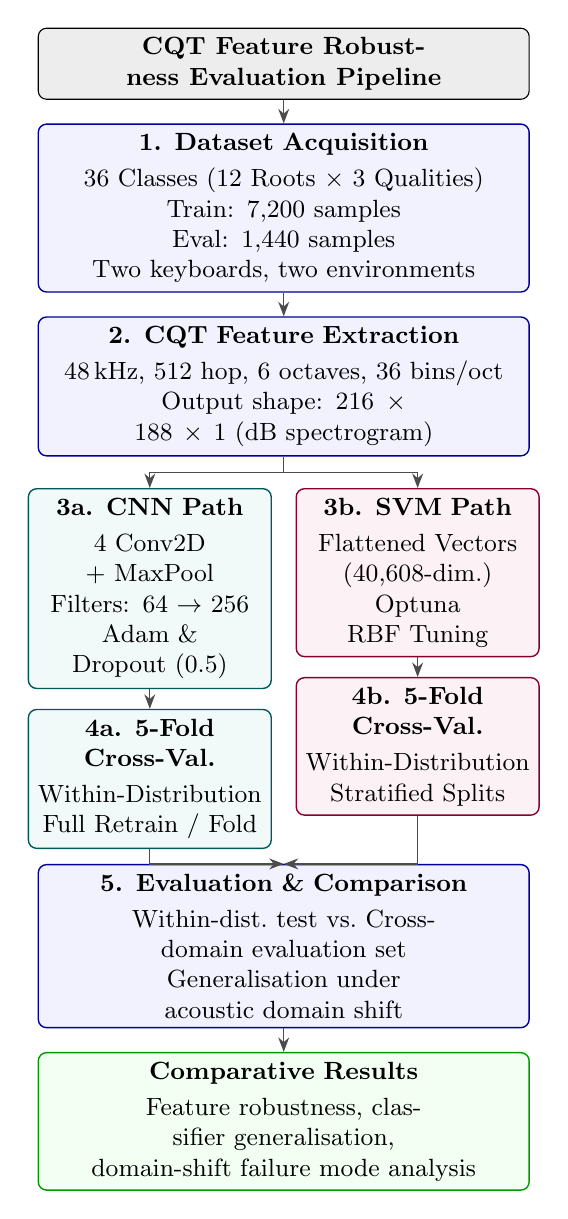
\begin{tikzpicture}[
  node distance=0.3cm and 0.2cm,
  >={Stealth},
  base/.style={
    rectangle, draw, align=center,
    minimum height=0.6cm,
    font=\small,
    rounded corners=3pt,
    line width=0.5pt
  },
  main/.style={
    base,
    draw=blue!60!black,
    fill=blue!5,
    text width=6.0cm
  },
  cnn/.style={
    base,
    draw=teal!70!black,
    fill=teal!5,
    text width=2.85cm
  },
  svm/.style={
    base,
    draw=purple!70!black,
    fill=purple!5,
    text width=2.85cm
  },
  clear/.style={
    base,
    draw=green!60!black,
    fill=green!5,
    text width=6.0cm,
    font=\small
  },
  arrow/.style={->, line width=0.5pt, black!70}
]

%% Header
\node[draw, rounded corners=3pt, fill=black!7,
      text width=6.0cm, align=center,
      font=\small\bfseries, minimum height=0.45cm]
  (header) {CQT Feature Robustness Evaluation Pipeline};

%% Phase 1
\node[main, below=0.3cm of header] (p1) {%
  \textbf{1. Dataset Acquisition}\\[2pt]
  36 Classes (12 Roots $\times$ 3 Qualities)\\
  Train: 7{,}200 samples \quad Eval: 1{,}440 samples\\
  Two keyboards, two environments
};

%% Phase 2
\node[main, below=0.3cm of p1] (p2) {%
  \textbf{2. CQT Feature Extraction}\\[2pt]
  48\,kHz, 512 hop, 6 octaves, 36 bins/oct\\
  Output shape: $216 \times 188 \times 1$ (dB spectrogram)
};

%% --- Parallel columns ---
\node[cnn, below left=0.4cm and 0.15cm of p2.south,
      anchor=north east] (cnn1) {%
  \textbf{3a. CNN Path}\\[2pt]
  4 Conv2D + MaxPool\\
  Filters: 64 $\to$ 256\\
  Adam \& Dropout (0.5)
};

\node[cnn, below=0.25cm of cnn1] (cnn2) {%
  \textbf{4a. 5-Fold Cross-Val.}\\[2pt]
  Within-Distribution\\
  Full Retrain / Fold
};

\node[svm, below right=0.4cm and 0.15cm of p2.south,
      anchor=north west] (svm1) {%
  \textbf{3b. SVM Path}\\[2pt]
  Flattened Vectors\\
  (40{,}608-dim.)\\
  Optuna RBF Tuning
};

\node[svm, below=0.25cm of svm1] (svm2) {%
  \textbf{4b. 5-Fold Cross-Val.}\\[2pt]
  Within-Distribution\\
  Stratified Splits
};

%% Phase 5
\node[main,
      below=0.4cm of $(cnn2.south)!0.5!(svm2.south)$,
      anchor=north] (p5) {%
  \textbf{5. Evaluation \& Comparison}\\[2pt]
  Within-dist.\ test vs.\ Cross-domain evaluation set\\
  Generalisation under acoustic domain shift
};

%% Final output
\node[clear, below=0.3cm of p5] (res) {%
  \textbf{Comparative Results}\\[2pt]
  Feature robustness, classifier generalisation,\\
  domain-shift failure mode analysis
};

%% --- Arrows ---
\draw[arrow] (header) -- (p1);
\draw[arrow] (p1)     -- (p2);

\draw[arrow] (p2.south) -- ++(0,-0.2) -| (cnn1.north);
\draw[arrow] (p2.south) -- ++(0,-0.2) -| (svm1.north);

\draw[arrow] (cnn1) -- (cnn2);
\draw[arrow] (svm1) -- (svm2);

\draw[arrow] (cnn2.south) -- ++(0,-0.2) |- (p5.north);
\draw[arrow] (svm2.south) -- ++(0,-0.2) |- (p5.north);

\draw[arrow] (p5) -- (res);

\end{tikzpicture}
\caption{Experimental pipeline for CQT feature robustness and classifier
generalisation evaluation. Both classifiers operate on identical CQT
features. The pipeline separates within-distribution cross-validation
from cross-domain evaluation to isolate the effect of acoustic domain
shift on classifier generalisation.}
\label{fig:methodology}
\end{figure}

\subsection{Dataset Acquisition}\label{subsec3_1}

\subsubsection{Acquisition Method}\label{subsubsec3_1_1}

Audio recordings are collected using a custom web-based MIDI recording
application developed specifically for this study (Fig.~\ref{fig3_1}).
The application connects to a keyboard instrument via USB MIDI,
programmatically triggers chords by sending simultaneous MIDI note-on
events for each chord constituent, and captures the resulting audio
through a connected microphone.
This deterministic triggering approach eliminates manual playing errors
and produces recordings with organic acoustic properties arising from the
instrument's physical resonance and synthesis, while maintaining
consistent chord content across all recordings.

\begin{figure}[h]
\centering
\includegraphics[width=\columnwidth]{Fig1.png}
\caption{Web application used to generate and record the dataset.
The interface connects to a keyboard via USB MIDI, triggers chord note
events programmatically, and records the resulting audio.}
\label{fig3_1}
\end{figure}

\subsubsection{Chord Vocabulary}\label{subsubsec3_1_2}

The chord vocabulary covers 36 classes formed by the combination of
12 chromatic root notes (C, C$\sharp$, D, D$\sharp$, E, F, F$\sharp$,
G, G$\sharp$, A, A$\sharp$, B) and 3 chord quality types (major, minor,
diminished).
All chords are voiced in the fourth octave, which provides optimal
spectral coverage within the 6-octave CQT range and clear harmonic
separability between qualities \cite{Telila2023} \cite{Harte2010}.
The inclusion of the diminished quality tests classifier sensitivity to
a harmonically dense chord type in which all intervals are minor thirds,
creating greater inter-class harmonic proximity than major or minor
chords \cite{Aidinis2024}.
The selected vocabulary, while smaller than large-scale ACR benchmarks,
is appropriate for controlled generalisation analysis because the classes
are well-characterised, the feature structure is geometrically regular,
and the inter-class boundaries are well-defined in CQT frequency space.

\subsubsection{Dataset Split and Recording Conditions}\label{subsubsec3_1_3}

Two independent datasets are recorded to enable cross-domain evaluation:

\begin{enumerate}[1.]

\item \textbf{Training dataset}: 200 samples per class, 7,200 total.
Recorded using a Xiaomi Redmi Pad 2 microphone from a Techno T-9890i
keyboard with Acoustic Grand Piano voice.
Note attack delays are randomised in the range 0--150\,ms to simulate
natural playing articulation and prevent overfitting to perfectly
synchronous note onsets.

\item \textbf{Evaluation dataset}: 40 samples per class, 1,440 total.
Recorded using the internal microphone of an ASUS ROG Flow X13 laptop
from a Yamaha PSR-S910 keyboard with Grand Piano voice, in a different
physical room.
Note attack delays are randomised in the range 0--100\,ms.
Half of the samples per class are recorded at a relatively higher input
volume level to introduce additional inter-sample acoustic variation.

\end{enumerate}

The two datasets differ systematically in instrument brand, piano voice
synthesis algorithm, recording device, microphone frequency response,
and physical recording environment.
No samples from the evaluation dataset were used at any stage of
training, validation, or hyperparameter optimisation.
This strict separation ensures that cross-domain results measure
genuine out-of-distribution generalisation.
All recordings are stored in OGG/OPUS format at 48,000\,Hz sample rate,
32-bit depth, mono channel, without post-processing filters.
The distribution of audio durations across the training dataset is
shown in Fig.~\ref{fig3_2}.

\begin{figure}[h]
\centering
\includegraphics[width=\columnwidth]{Fig2.eps}
\caption{Audio duration distribution across classes in the training
dataset. Variation in duration arises from the randomised note attack
delays of 0--150\,ms applied during recording.}
\label{fig3_2}
\end{figure}

\subsection{CQT Feature Extraction}\label{subsec3_2}

Feature extraction is performed using the Constant-Q Transform via the
\texttt{librosa.cqt()} function \cite{McFee2025}.
The CQT computes a time-frequency representation in which each
frequency bin $f_k$ satisfies a constant quality factor:

\begin{equation}
Q = \frac{f_k}{f_{k+1} - f_k} = \frac{1}{2^{1/B} - 1}
\label{eq:cqt}
\end{equation}

where $B$ is the number of bins per octave \cite{Li2021} \cite{Lacoste2007}.
This logarithmic frequency spacing directly aligns each bin with a
musical semitone, making the resulting 2D spectrogram invariant to chord
transposition and producing geometrically consistent harmonic patterns
regardless of root pitch — an inductive bias that benefits both CNN
pattern recognition and classification across instruments \cite{Li2021}
\cite{Telila2023}.

The extraction parameters are summarised in Table~\ref{tab1}.
The configuration of 36 bins per octave (3 bins per semitone) provides
frequency resolution sufficient to resolve the harmonic interval
differences between major ($+4, +3$ semitones), minor ($+3, +4$
semitones), and diminished ($+3, +3$ semitones) triads, consistent
with prior work by Akram et al.\ \cite{Akram2025}, O'Hanlon and Sandler
\cite{OHanlon2021}, and Rowe and Tzanetakis \cite{Rowe2021}.

\begin{table}[h]
\caption{CQT feature extraction parameters}
\label{tab1}
\begin{tabular}{@{}ll@{}}
\toprule
Parameter          & Value \\
\midrule
Sample Rate        & 48{,}000\,Hz \\
Hop Size           & 512 samples \\
Number of Octaves  & 6 \\
Bins per Octave    & 36 \\
Total Frequency Bins & 216 \\
Lowest Frequency   & C1 (32.70\,Hz) \\
Highest Frequency  & C7 (2{,}093\,Hz) \\
Window Function    & Hann \\
Fixed Frame Length & 188 frames \\
Output Shape       & $216 \times 188 \times 1$ \\
\bottomrule
\end{tabular}
\end{table}

Each audio sample is truncated or zero-padded to a fixed duration of
2.0\,seconds prior to feature extraction, corresponding to the minimum
recording duration observed across the dataset (see Fig.~\ref{fig3_2}).
The fixed frame length of 188 is derived as:

\begin{equation}
\text{frames} = \left\lfloor\frac{\text{duration} \times f_s}{\text{hop size}}\right\rfloor
= \left\lfloor\frac{2.0 \times 48{,}000}{512}\right\rfloor = 187 \approx 188
\label{eq:frames}
\end{equation}

The output of the CQT extraction for each sample is a $216 \times 188$
matrix of magnitude values in decibels (dB), where rows correspond to
frequency bins (C1 to C7) and columns correspond to time frames
(0 to 1.999\,s).
This representation simultaneously captures pitch-axis harmonic structure
and time-axis onset/decay dynamics, providing a rich 2D feature map
for convolutional processing.

\subsection{CNN Architecture and Training}\label{subsec3_3}

\subsubsection{Architecture}\label{subsubsec3_3_1}

The CNN architecture is adapted from Wolf-Monheim
\cite{Wolf-Monheim2024}\cite{Wolf-Monheim2025}, originally designed for
environmental sound classification using spectral features on the ESC-50
dataset \cite{Purwono2022}.
The architecture was selected for its compact four-block convolutional
structure without recurrent layers, attention mechanisms, or secondary
temporal models, which is appropriate for fixed-window classification
from static spectrograms.
Table~\ref{tab2} specifies the complete layer sequence.

\begin{table*}[h]
\caption{CNN architecture specification for 36-class CQT spectrogram classification}
\label{tab2}
\begin{tabular*}{\textwidth}{@{\extracolsep\fill}lll}
\toprule
Layer               & Output Shape              & Parameters / Notes \\
\midrule
BatchNormalization  & $216 \times 188 \times 1$ & Normalises input CQT dB values \\
Conv2D              & $216 \times 188 \times 64$  & $3\times3$, ReLU, same padding \\
MaxPooling2D        & $108 \times 94 \times 64$   & $2\times2$, stride 2 \\
Conv2D              & $108 \times 94 \times 128$  & $3\times3$, ReLU, same padding \\
MaxPooling2D        & $54 \times 47 \times 128$   & $2\times2$, stride 2 \\
Conv2D              & $54 \times 47 \times 256$   & $3\times3$, ReLU, same padding \\
MaxPooling2D        & $27 \times 23 \times 256$   & $2\times2$, stride 2 \\
Conv2D              & $27 \times 23 \times 256$   & $3\times3$, ReLU, same padding \\
MaxPooling2D        & $13 \times 11 \times 256$   & $2\times2$, stride 2 \\
Flatten             & 36{,}608                    & — \\
Dense               & 256                         & ReLU activation \\
Dropout             & 256                         & rate $= 0.5$ \\
Dense (Output)      & 36                          & Softmax activation \\
\bottomrule
\end{tabular*}
\end{table*}

Input batch normalisation ensures consistent CQT magnitude statistics
across samples and recording conditions, which is particularly important
for cross-domain robustness since different recording environments may
produce different absolute magnitude ranges \cite{Purwono2022}.
The four successive Conv2D-MaxPooling2D blocks build a progressive
feature hierarchy: the first block (64 filters) captures low-level
spectral texture features; the second block (128 filters) encodes
mid-level harmonic interval patterns; the third and fourth blocks
(256 filters each) represent high-level chord quality abstractions.
The $3\times3$ convolutional receptive field is well-matched to the
bin-level CQT interval differences between chord types (1--2 bins per
semitone transition), enabling localised detection of major-to-minor
and minor-to-diminished quality differences \cite{OShea2015}.
MaxPooling provides spatial subsampling and limited translation
invariance, reducing sensitivity to small spectral shifts \cite{Purwono2022}.
The Dropout layer (rate $= 0.5$) prevents co-adaptation during training
and serves as an implicit regulariser against overfitting to the specific
timbral characteristics of the training instrument.

\subsubsection{Training Configuration}\label{subsubsec3_3_2}

Training parameters are summarised in Table~\ref{tab3}.

\begin{table}[h]
\caption{CNN training configuration}
\label{tab3}
\begin{tabularx}{\columnwidth}{@{}lX@{}}
\toprule
Parameter                   & Value \\
\midrule
Random State                & 42 \\
Training Partition          & 80\% (5{,}760 samples) \\
Validation Partition        & 10\% (720 samples) \\
Test Partition              & 10\% (720 samples) \\
Batch Size                  & 32 \\
Initial Learning Rate       & 0.001 \\
Optimiser                   & Adam \\
Weight Initialisation       & Glorot (Xavier) uniform \\
Loss Function               & Categorical cross-entropy \\
Maximum Epochs              & 50 \\
EarlyStopping patience      & 6 epochs (validation loss) \\
ReduceLROnPlateau           & factor 0.1, patience 2 epochs \\
\bottomrule
\end{tabularx}
\end{table}

Stratified random sampling with a fixed seed of 42 is used for all data
splits to ensure balanced class representation and full reproducibility.
Glorot (Xavier) uniform weight initialisation ensures that gradient
variance is preserved through the network depth at initialisation
\cite{Purwono2022}.
The ReduceLROnPlateau callback reduces the learning rate by a factor of
0.1 when validation loss stagnates for 2 epochs, enabling fine-grained
convergence near the loss minimum.
EarlyStopping terminates training after 6 consecutive epochs without
validation loss improvement and saves the best-performing weights.
The final model evaluation uses the 10\% held-out test partition, which
is entirely excluded from all training and validation phases.

\subsection{5-Fold Cross-Validation}\label{subsec3_4}

Stratified 5-fold cross-validation is performed on the full 7,200-sample
training dataset to assess the statistical robustness of within-distribution
classification performance independently of a single train/test split.
In each fold, 80\% of the data is allocated to training and 20\% to
testing.
Each fold involves a complete re-initialisation and re-training of the
CNN from scratch with a fixed random seed per fold.
For the SVM, each fold evaluates the final optimised model on the
corresponding fold test partition.
This procedure provides five independent performance measurements that
collectively characterise the within-distribution generalisation capacity
of each classifier.

\subsection{SVM Hyperparameter Optimisation}\label{subsec3_5}

An RBF-kernel SVM is configured as a comparative classifier using
scikit-learn's SVC implementation \cite{Pedregosa2011}.
Identical CQT features are used as input to both classifiers to ensure
a fair comparison of architecture effects in isolation from feature
differences.
Because SVM requires a flattened input, each $216 \times 188$ CQT matrix
is reshaped into a 40,608-dimensional vector prior to classification.

Hyperparameter optimisation is conducted using Optuna \cite{Akiba2019}
with a RandomSampler over 10 trials.
The search space follows Chang and Lin \cite{Chang2011} and Wainer and
Fonseca \cite{Wainer2020}: $C \in \{0.1, 1, 10, 100, 1000\}$,
$\gamma \in \{10^{-6}, 10^{-5}, 10^{-4}, 10^{-3}\}$.
Each trial is evaluated using stratified 5-fold cross-validation accuracy
on the training dataset.
This exhaustive search over the recommended parameter grid ensures that
the SVM baseline achieves optimal within-distribution performance before
cross-domain evaluation.

\subsection{Evaluation Metrics}\label{subsec3_6}

Classification performance is evaluated using the standard metrics
derived from the confusion matrix \cite{Hossin2015}.
For a binary partition of one class against all others, the four
fundamental quantities are True Positives (TP), True Negatives (TN),
False Positives (FP), and False Negatives (FN).
The metrics are defined as follows:

\begin{equation}
\text{Accuracy} = \frac{TP + TN}{TP + FP + TN + FN}
\label{eq:acc}
\end{equation}

\begin{equation}
\text{Precision} = \frac{TP}{TP + FP}
\label{eq:prec}
\end{equation}

\begin{equation}
\text{Recall} = \frac{TP}{TP + FN}
\label{eq:rec}
\end{equation}

\begin{equation}
\text{F1\text{-}score} = \frac{2 \times \text{Precision} \times \text{Recall}}{\text{Precision} + \text{Recall}}
\label{eq:f1}
\end{equation}

For 36-class classification, macro-averaged precision, recall, and
F1-score are reported, assigning equal weight to each class regardless
of sample count.
Macro averaging is the appropriate aggregation for generalisation
analysis, as it penalises class-level failure equally regardless of
class frequency — in contrast to weighted averaging, which can inflate
apparent performance when a small number of dominant classes are
classified correctly.

%% -----------------------------------------------------------------------
\section{Results and Discussion}\label{sec4}
%% -----------------------------------------------------------------------

\subsection{CQT Feature Extraction}\label{subsec4_1}

Feature extraction transforms all 8,640 audio recordings (7,200 training,
1,440 evaluation) into $216 \times 188$ CQT decibel matrices.
Figure~\ref{fig4_1} shows representative extracted spectrograms from
four training dataset classes.
The spectrograms visibly encode qualitatively distinct harmonic patterns:
major and minor chords of the same root show a vertical offset of one
frequency bin in the third overtone row, while diminished chords display
a compressed, more uniform energy distribution across the harmonic rows.
These inter-class spectral differences are geometrically consistent across
the frequency axis, confirming that CQT features embed the harmonic
structure of chords in a spatially regular form that is well-suited for
convolutional pattern recognition.

\begin{figure}[h]
\centering
\includegraphics[width=\columnwidth]{Fig3.eps}
\caption{Representative CQT spectrogram samples extracted from the
training dataset. From left to right: D$\sharp$\_diminished\_4,
A\_diminished\_4, E\_minor\_4, F\_diminished\_4. Harmonic structure
differences between chord qualities are visible as consistent
frequency-axis patterns.}
\label{fig4_1}
\end{figure}

The consistency of these patterns across the training dataset
(200 samples per class, 7,200 total) establishes that the
within-distribution feature space provides sufficient and unambiguous
class-separating information for both the CNN and SVM classifiers.
The question of whether this separability is preserved when the same
CQT parameters are applied to audio from a different instrument is
addressed in Section~\ref{subsec4_4}.

\subsection{CNN Training and Within-Distribution Evaluation}\label{subsec4_2}

\subsubsection{Training Dynamics}\label{subsubsec4_2_1}

As shown in Fig.~\ref{fig4_2}, the CNN model exhibits rapid and stable
convergence.
Training accuracy increases from 47.65\% at epoch 1 to 98.41\% at
epoch 2 and reaches a peak of 99.91\% at epoch 8.
Validation accuracy reaches 99.85\% at epoch 2 and achieves 100\%
by epoch 3.
EarlyStopping is triggered after epoch 10, saving the best weights from
epoch 4.

\begin{figure}[h]
\centering
\includegraphics[width=\columnwidth]{Fig4.eps}
\caption{CNN training and validation accuracy and loss over training
epochs. Rapid convergence is observed by epoch 2--3, consistent with
the high discriminability of CQT features for within-distribution
chord classification.}
\label{fig4_2}
\end{figure}

The characteristic gap between training accuracy (limited by dropout
stochasticity during training) and validation accuracy (evaluated with
dropout disabled) during early epochs is consistent with a
well-regularised model.
The absence of divergence between training and validation loss
throughout training confirms that no significant overfitting occurred.
Rapid convergence is consistent with the well-structured, harmonically
separable nature of within-distribution CQT features.

After training, evaluation on the 10\% held-out test partition (720
samples, 20 per class) yields perfect classification accuracy, precision,
recall, and F1-score of 1.0000.
The confusion matrix (Fig.~\ref{fig4_3}) shows a fully filled diagonal,
indicating zero misclassifications across all 36 classes.

\begin{figure}[h]
\centering
\includegraphics[width=\columnwidth]{Fig5.eps}
\caption{CNN test set confusion matrix (within-distribution, 720 samples,
20 per class). Perfect diagonal dominance confirms zero misclassifications
across all 36 chord classes.}
\label{fig4_3}
\end{figure}

This result confirms that the combination of 36-bin/octave CQT spectrograms
and the four-block CNN architecture is sufficient to achieve perfect
within-distribution discrimination for the 36-class piano chord vocabulary.
The $3\times3$ convolutional kernels, applied at four spatial scales,
effectively capture the 1--2 bin frequency shifts that distinguish major,
minor, and diminished chord qualities at this CQT resolution.

\subsubsection{5-Fold Cross-Validation}\label{subsubsec4_2_2}

Table~\ref{tab4_1} presents the CNN 5-fold cross-validation results.

\begin{table*}[h]
\caption{CNN 5-fold cross-validation results (within-distribution)}
\label{tab4_1}
\begin{tabular*}{\textwidth}{@{\extracolsep\fill}llllllll}
\toprule
 & & \multicolumn{3}{l}{Accuracy} & \multicolumn{3}{l}{Loss} \\
\cmidrule(lr){3-5} \cmidrule(lr){6-8}
Fold & Epochs & Train & Validation & Test & Train & Validation & Test \\
\midrule
Fold 1 & 11 & 0.9979 & 1.0000 & 1.0000 & 0.0051 & 0.0000 & 0.0003 \\
Fold 2 & 21 & 0.9979 & 1.0000 & 1.0000 & 0.0051 & 0.0000 & 0.0000 \\
Fold 3 & 19 & 0.9969 & 1.0000 & 1.0000 & 0.0063 & 0.0000 & 0.0000 \\
Fold 4 & 15 & 0.9967 & 1.0000 & 1.0000 & 0.0091 & 0.0000 & 0.0000 \\
Fold 5 & 14 & 0.9985 & 1.0000 & 1.0000 & 0.0058 & 0.0000 & 0.0001 \\
Mean   & 16.0 & 0.9976 & 1.0000 & 1.0000 & 0.0074 & 0.0000 & 0.0001 \\
Std.   & 3.58 & 0.0007 & 0.0000 & 0.0000 & 0.0020 & 0.0000 & 0.0001 \\
\bottomrule
\end{tabular*}
\end{table*}

Across all five folds, the CNN achieves perfect validation and test
accuracy (1.0000) with zero standard deviation, confirming that the
result is not an artefact of a particular data split.
Mean training accuracy of 0.9976 with a standard deviation of 0.0007
reflects only the stochastic effect of dropout during training, which
does not affect test performance.
The mean test loss of 0.0001 indicates that the model's output probability
distributions are sharply concentrated on the correct class throughout.
These results are visualised in Fig.~\ref{fig4_4}.

\begin{figure}[h]
\centering
\includegraphics[width=\columnwidth]{Fig6.eps}
\caption{CNN 5-fold cross-validation training curves. Consistent
rapid convergence and perfect test accuracy across all five folds
confirm that within-distribution CQT features are fully separable
by the CNN architecture.}
\label{fig4_4}
\end{figure}

The zero cross-fold variance provides strong statistical evidence that
the CNN's learned decision boundaries are stable across different random
data partitions, ruling out data split bias as an alternative explanation
for the high accuracy.

\subsection{SVM Hyperparameter Optimisation and Within-Distribution Evaluation}\label{subsec4_3}

\subsubsection{Hyperparameter Optimisation}\label{subsubsec4_3_1}

As shown in Fig.~\ref{fig4_5}, Optuna's RandomSampler converges at
trial 7 with optimal parameters $C = 1000$ and
$\gamma = 10^{-5}$.
At this configuration, the SVM achieves perfect validation accuracy,
triggering early termination of the search.

\begin{figure}[h]
\centering
\includegraphics[width=\columnwidth]{Fig7.eps}
\caption{SVM Optuna hyperparameter search results. Convergence at
trial 7 with $C = 1000$, $\gamma = 10^{-5}$ confirms that the
search space contains the globally optimal configuration for
within-distribution classification.}
\label{fig4_5}
\end{figure}

The optimised SVM (C = 1000, $\gamma = 10^{-5}$) achieves perfect
accuracy (1.000) on the 10\% test partition, with a confusion matrix
(Fig.~\ref{fig4_6}) showing zero misclassifications.
The high value of the regularisation parameter $C$ indicates that the
optimal SVM boundary is a hard-margin or near-hard-margin solution on
the training data, which is consistent with the high discriminability
of within-distribution CQT features in the 40,608-dimensional feature
space.

\begin{figure}[h]
\centering
\includegraphics[width=\columnwidth]{Fig8.eps}
\caption{SVM test set confusion matrix (within-distribution, 720 samples).
Zero misclassifications confirm that the 40,608-dimensional flattened
CQT feature space provides a linearly separable representation for
the optimised RBF kernel.}
\label{fig4_6}
\end{figure}

\subsubsection{5-Fold Cross-Validation}\label{subsubsec4_3_2}

Table~\ref{tab4_2} presents the SVM 5-fold cross-validation results.

\begin{table}[h]
\caption{SVM 5-fold cross-validation results (within-distribution)}
\label{tab4_2}
\begin{tabular}{@{}lllll@{}}
\toprule
Fold    & Accuracy & Macro F1 & Weighted F1 \\
\midrule
Fold 1  & 1.0000 & 1.0000 & 1.0000 \\
Fold 2  & 1.0000 & 1.0000 & 1.0000 \\
Fold 3  & 1.0000 & 1.0000 & 1.0000 \\
Fold 4  & 1.0000 & 1.0000 & 1.0000 \\
Fold 5  & 1.0000 & 1.0000 & 1.0000 \\
Mean    & 1.0000 & 1.0000 & 1.0000 \\
Std.    & 0.0000 & 0.0000 & 0.0000 \\
\bottomrule
\end{tabular}
\end{table}

The SVM achieves perfect accuracy and F1-score across all five folds
with zero variance, identical to the CNN under the same conditions.
This result is significant: it demonstrates that the CQT features are
so discriminative within the training distribution that even a global
kernel classifier can achieve zero errors.
The SVM's perfect within-distribution performance rules out any
explanation for subsequent cross-domain failure based on insufficient
model capacity or suboptimal hyperparameters — the failure, when it
occurs, is structural rather than configural.

\subsection{Within-Distribution Comparative Summary}\label{subsec4_4}

Table~\ref{tab4_3} summarises the within-distribution performance of
both classifiers.

\begin{table}[h]
\caption{CNN vs.\ SVM within-distribution comparison (5-fold cross-validation)}
\label{tab4_3}
\begin{tabular}{@{}lllll@{}}
\toprule
 & \multicolumn{2}{l}{CNN} & \multicolumn{2}{l}{SVM} \\
\cmidrule(lr){2-3} \cmidrule(lr){4-5}
Fold   & Accuracy & F1-Score & Accuracy & F1-Score \\
\midrule
Fold 1 & 1.0000 & 1.0000 & 1.0000 & 1.0000 \\
Fold 2 & 1.0000 & 1.0000 & 1.0000 & 1.0000 \\
Fold 3 & 1.0000 & 1.0000 & 1.0000 & 1.0000 \\
Fold 4 & 1.0000 & 1.0000 & 1.0000 & 1.0000 \\
Fold 5 & 1.0000 & 1.0000 & 1.0000 & 1.0000 \\
Mean   & 1.0000 & 1.0000 & 1.0000 & 1.0000 \\
Std.   & 0.0000 & 0.0000 & 0.0000 & 0.0000 \\
\bottomrule
\end{tabular}
\end{table}

Under within-distribution conditions, CNN and SVM produce
indistinguishable results: both achieve perfect accuracy and F1-score
with zero variance across all five folds.
This equivalence is a key experimental finding: it establishes that
the CQT feature representation is \emph{necessary and sufficient} for
the within-distribution task, irrespective of the classifier.
CNN's added architectural complexity yields no measurable benefit when
the feature space is fully discriminative and acoustically stable.
This parity shifts the analytical focus to the cross-domain evaluation
in Section~\ref{subsec4_5}, where the structural differences between
the classifiers become decisive.

\subsection{Cross-Domain Evaluation}\label{subsec4_5}

\subsubsection{CNN on the Evaluation Dataset}\label{subsubsec4_5_1}

The trained CNN is evaluated on the 1,440-sample evaluation dataset
recorded from a Yamaha PSR-S910 keyboard in a different physical
environment.
No fine-tuning or domain adaptation is applied; the model evaluated is
identical to the one obtained from within-distribution training.

The resulting confusion matrix (Fig.~\ref{fig4_7}) shows that the CNN
retains substantial predictive capability across the domain shift.
The majority of chord classes are classified with perfect or near-perfect
accuracy (40/40 correct), including all B, C$\sharp$, D$\sharp$, D,
F$\sharp$, F, G, and G$\sharp$ major and minor classes.
Misclassifications are not distributed randomly across all classes but
are systematically concentrated in a small set of harmonically proximate
chord pairs, as detailed in Table~\ref{tab4_4}.

\begin{figure}[h]
\centering
\includegraphics[width=\columnwidth]{Fig9.eps}
\caption{CNN confusion matrix on the cross-domain evaluation dataset
(1,440 samples, 40 per class). Diagonal dominance is maintained
across most classes; misclassifications are concentrated in a small
number of harmonically related chord pairs.}
\label{fig4_7}
\end{figure}

\begin{table}[h]
\caption{CNN misclassification analysis on the evaluation dataset}
\label{tab4_4}
\begin{tabular}{@{}lll@{}}
\toprule
True Class               & Predicted Class             & Count \\
\midrule
A\_diminished\_4         & A$\sharp$\_major\_4         & 20 \\
C\_diminished\_4         & C$\sharp$\_diminished\_4    & 16 \\
E\_diminished\_4         & F\_diminished\_4            & 10 \\
E\_diminished\_4         & D$\sharp$\_diminished\_4    &  7 \\
F$\sharp$\_major\_4      & G$\sharp$\_major\_4         &  5 \\
F$\sharp$\_minor\_4      & F$\sharp$\_diminished\_4    &  5 \\
G$\sharp$\_minor\_4      & G$\sharp$\_diminished\_4    &  4 \\
E\_minor\_4              & F$\sharp$\_diminished\_4    &  3 \\
B\_major\_4              & A$\sharp$\_major\_4         &  2 \\
B\_major\_4              & F$\sharp$\_major\_4         &  2 \\
D$\sharp$\_diminished\_4 & C$\sharp$\_diminished\_4    &  2 \\
A$\sharp$\_major\_4      & A$\sharp$\_minor\_4         &  1 \\
A\_major\_4              & B\_minor\_4                 &  1 \\
C\_major\_4              & D$\sharp$\_major\_4         &  1 \\
D\_minor\_4              & C$\sharp$\_minor\_4         &  1 \\
F$\sharp$\_minor\_4      & E$\sharp$\_minor\_4         &  1 \\
\bottomrule
\end{tabular}
\end{table}

Three features of this misclassification pattern are diagnostically
informative.
First, the largest single error (A\_diminished $\to$ A$\sharp$\_major,
20 counts) involves a quality shift from diminished to major combined
with a semitone root displacement, a confusion consistent with a global
downward frequency shift of the evaluation instrument's spectral
envelope causing the CQT pattern of A\_diminished to shift into the
neighbourhood of A$\sharp$\_major.
Second, the next largest error cluster (C\_diminished $\to$
C$\sharp$\_diminished, 16 counts) is a pure semitone root shift with
preserved quality, again consistent with a global frequency offset.
Third, all remaining errors involve either neighbouring semitone roots
or adjacent qualities (major $\leftrightarrow$ minor,
minor $\leftrightarrow$ diminished) — never large-interval confusions
across unrelated classes.

This error topology is consistent with the CNN having learned CQT
interval patterns (relative frequency offsets between root, third, and
fifth) that are partially robust to global spectral shifts, but failing
at boundary cases where the shift moves the test pattern across a
class boundary defined by a single semitone.
The overall accuracy of 0.89 and macro F1-score of 0.87 on 1,440
cross-domain samples demonstrate that the CNN's local hierarchical
feature learning generalises meaningfully beyond the training domain.

\subsubsection{SVM on the Evaluation Dataset}\label{subsubsec4_5_2}

The optimised RBF-SVM is evaluated under identical cross-domain
conditions.
The resulting confusion matrix (Fig.~\ref{fig4_8}) reveals severe
generalisation failure.

\begin{figure}[h]
\centering
\includegraphics[width=\columnwidth]{Fig10.eps}
\caption{SVM confusion matrix on the cross-domain evaluation dataset
(1,440 samples). The near-complete concentration of predictions on
a single class (C\_diminished\_4) constitutes a model collapse under
acoustic domain shift.}
\label{fig4_8}
\end{figure}

The SVM overwhelmingly predicts C\_diminished\_4 for the large majority
of test samples regardless of the true label, a pattern diagnostic of
a \emph{single-class attractor}.
This failure mode arises because the RBF kernel measures the Euclidean
distance between a test sample's 40,608-dimensional flattened CQT
vector and the training support vectors.
When the Yamaha PSR-S910's different piano voice synthesis produces CQT
feature vectors with a globally shifted spectral envelope — due to
different harmonic series weights, different attack/decay characteristics,
and a different microphone transfer function — the distances to all
support vectors are systematically altered.
Under this shift, a large portion of the evaluation samples fall closest,
in kernel distance, to the support vectors of C\_diminished\_4, which
acts as a global attractor in the mismatched feature space.
The SVM achieves cross-domain accuracy of 0.29 and macro F1-score of 0.36.

\subsubsection{Comparative Analysis and Generalisation Mechanisms}\label{subsubsec4_5_3}

Figure~\ref{fig4_9} visualises the metric divergence between the two
classifiers on the evaluation dataset.
Table~\ref{tab4_5} presents the complete comparative summary across
within-distribution and cross-domain conditions.

\begin{figure}[h]
\centering
\includegraphics[width=\columnwidth]{Fig11.eps}
\caption{CNN vs.\ SVM performance comparison across within-distribution
(cross-validation) and cross-domain (evaluation dataset) conditions.
Under within-distribution evaluation both classifiers achieve perfect
scores; under cross-domain evaluation the CNN maintains high performance
while the SVM collapses.}
\label{fig4_9}
\end{figure}

\begin{table*}[h]
\caption{CNN vs.\ SVM full comparative results across within-distribution and cross-domain evaluation}
\label{tab4_5}
\begin{tabular*}{\textwidth}{@{\extracolsep\fill}lllllll}
\toprule
 & \multicolumn{3}{l}{CNN} & \multicolumn{3}{l}{SVM} \\
\cmidrule(lr){2-4} \cmidrule(lr){5-7}
Metric    & Training CV & Test & Evaluation
          & Training CV & Test & Evaluation \\
\midrule
Accuracy  & 1.00 & 1.00 & 0.89 & 1.00 & 1.00 & 0.29 \\
Precision & 1.00 & 1.00 & 0.91 & 1.00 & 1.00 & 0.64 \\
Recall    & 1.00 & 1.00 & 0.89 & 1.00 & 1.00 & 0.29 \\
F1-Score  & 1.00 & 1.00 & 0.87 & 1.00 & 1.00 & 0.36 \\
\bottomrule
\end{tabular*}
\end{table*}

The results in Table~\ref{tab4_5} exhibit a clear and interpretable
structure.
Under within-distribution evaluation, both models achieve perfect and
indistinguishable performance, confirming that the CQT feature space is
fully discriminative under consistent recording conditions and that both
classifier types are capable of learning the decision boundary.
The divergence under cross-domain evaluation is therefore entirely
attributable to the structural difference in how each classifier
generalises when the marginal feature distribution shifts — not to
differences in model capacity or optimisation quality.

The CNN's cross-domain accuracy of 0.89 and macro F1-score of 0.87
represent a reduction of 0.13 points from within-distribution
performance.
This reduction reflects the CNN's partial but meaningful preservation of
its learned spectral interval representations when the source of acoustic
variation (instrument timbre, recording device) changes.
The CNN's local convolutional receptive fields learn to detect relative
frequency interval patterns — the ratios between root, third, and fifth
across the CQT bin axis — that are \emph{partially} preserved across
instruments, even as absolute spectral amplitudes and envelope shapes
shift.

The SVM's cross-domain accuracy drop from 1.00 to 0.29 is more than
three times larger in magnitude and constitutes a qualitatively different
failure mode.
The precision-recall asymmetry of 0.64 vs.\ 0.29 characterises
single-class attractor behaviour: when the majority of predictions are
concentrated on C\_diminished\_4, the precision for that single class
remains high (correctly predicting the few true C\_diminished\_4 samples),
while recall collapses for all other 35 classes.
The macro F1-score of 0.36 is the most informative summary statistic in
this context, as it averages over all 36 classes equally: a classifier
predicting a single class uniformly would achieve a recall of
$1/36 \approx 0.028$ and a macro F1 close to zero, while the SVM's
partial retention of a few classes inflates this figure modestly above
zero while confirming near-total failure.

The precision-recall asymmetry and the single-attractor failure pattern
are both consistent with the theoretical prediction for RBF-SVM under
covariate shift: when the kernel bandwidth $\gamma = 10^{-5}$ is fixed
at a value calibrated to the training distribution, and the feature
distribution shifts by a global spectral offset, the Gaussian kernel
$k(\mathbf{x}, \mathbf{x}_i) = \exp(-\gamma \|\mathbf{x} - \mathbf{x}_i\|^2)$
becomes effectively zero for all support vectors except those whose
training features happen to be closest to the new distribution's centre
of mass.
The support vectors of C\_diminished\_4 evidently occupy this position
in the shifted feature space, producing the observed attractor.

These findings have implications extending beyond the specific domain of
piano chord classification.
Any spectrogram-based classification system deployed across varying
recording conditions — including environmental sound classifiers
\cite{Wolf-Monheim2025}, speaker identification systems
\cite{Zaman2023}, or bird call detectors — faces the same fundamental
trade-off: CNN's local spatial representations are more robust to global
spectral shifts than global kernel classifiers, but neither approach is
immune to domain shift.
The magnitude of the CNN's cross-domain accuracy (0.89) and the
nature of its residual errors (harmonic proximity confusions) suggest
that targeted data augmentation simulating inter-instrument timbral
variation and recording condition variation would be a tractable path
to closing the remaining performance gap.

%% -----------------------------------------------------------------------
\section{Conclusion}\label{sec5}
%% -----------------------------------------------------------------------

This paper presented a systematic evaluation of CQT spectrogram feature
robustness and classifier generalisation under acoustic domain shift,
using 36-class piano chord classification as a controlled experimental
platform.
The core experimental design — training on one keyboard instrument in
one environment and evaluating on a different instrument in a different
environment — explicitly isolates the effect of acoustic domain shift
on classifier performance.

The principal finding is a decisive divergence in cross-domain
generalisation between the two classifiers despite identical
within-distribution performance: CNN achieves 0.89 accuracy and 0.87
macro F1-score on the unseen evaluation dataset, while RBF-SVM collapses
to 0.29 accuracy and 0.36 macro F1-score through a single-class attractor
failure.
This divergence directly reflects the structural difference between
CNN's spatially local, hierarchical feature learning — which partially
preserves relative spectral interval patterns across the domain shift —
and RBF-SVM's global kernel boundary, which is rigidly calibrated to
the training feature distribution and cannot accommodate shifts in the
global spectral envelope.

A secondary finding is that within-distribution performance is not
predictive of cross-domain performance: the SVM's perfect
within-distribution accuracy provides no indication of its impending
collapse under domain shift.
This result reinforces the importance of cross-dataset or cross-condition
evaluation protocols in assessing spectrogram classifier deployability,
and argues against relying solely on held-out test splits from the same
recording session for performance reporting.

The CNN's residual misclassification pattern — concentrated in
harmonically proximate chord pairs separated by one semitone and
consistent with a global downward frequency shift of the evaluation
instrument's spectral envelope — provides actionable guidance for future
improvement.
Targeted data augmentation strategies that simulate inter-instrument
spectral envelope variation (pitch shifting, random spectral tilt,
time-varying equalization), combined with exposure to recordings from
a wider range of instruments during training, are predicted to
substantially reduce cross-domain error.
Extension of the chord vocabulary beyond fourth-octave triads and
integration of this classifier into a low-latency online recognition
pipeline remain further directions for future work.

More broadly, the experimental evidence supports the claim that
spatially local, hierarchically learned representations are more robust
to acoustic covariate shift than global kernel methods in the
spectrogram domain — a conclusion relevant to any application involving
CQT or other spectrogram-based classification under variable recording
conditions.

%% -----------------------------------------------------------------------
\backmatter
%% -----------------------------------------------------------------------

\bmhead{Author contributions}
All authors contributed to study conceptualisation and design. Material
preparation, data acquisition, experimentation, and analysis were
performed by Cikal Gemintang Seya. The first draft of the manuscript was
written by Cikal Gemintang Seya; all authors reviewed and approved the
final version.

\bmhead{Funding}
No funding was received for this work.

\bmhead{Data availability}
The piano chord dataset is publicly available at:
\url{https://zenodo.org/records/21077144} \cite{Seya2026}.

\bmhead{Code availability}
The dataset generation and recording tool is publicly available at:
\url{https://github.com/sglkc/chords-dataset-generator/}.

\section*{Declarations}

\bmhead{Conflict of interest}
The authors declare no competing interests.

\bmhead{Ethics approval}
Not applicable.

\bmhead{Consent for publication}
All authors approved the final manuscript.

\bibliography{mendeley}

\end{document}